\section{Âmbito do Produto}
\subsection{Fronteira do Produto}

Inserir aqui imagem do diagram geral de uc's !!!

\begin{comment}
\begin{figure}[!htb]
	\centering
	\includegraphics[scale=0.85]{images/diagramaGeralDeUseCase}
	\caption {Diagrama geral de \emph{Use Cases} do produto}
\end{figure}
\end{comment}


\subsection{Use Case Individuais do Produto}


\subsubsection{\textbf{1 - HoneyPot}}

Descrever aqui o uc do honeypot !!!
\begin{comment}
Qualquer utilizador do produto poderá efectuar uma simulação de seguro automóvel. No entanto, cada utlizador terá acesso a pequenas funcionalidades diferentes dependendo do tipo de utiliador em que se insere (registado ou não, mediador, etc). Aqui apresentaremos o fluxo normal deste \emph{use case} para um utilizador básico, ou seja, sem qualquer tipo de privilégios. Mais à frente, na explicação dos \emph{use cases} que se seguem, abordaremos as funcionalidades extra que cada tipo de utilizador terá. 
\end{comment}

\begin{figure}[!htb]
	\centering
	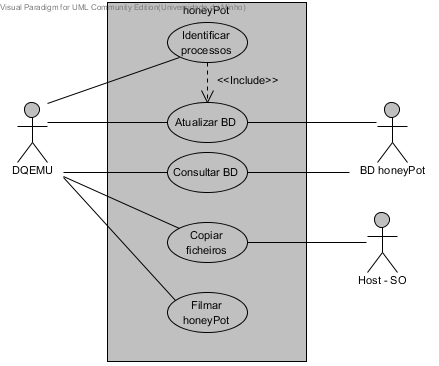
\includegraphics[scale=0.80]{images/ucs/HoneyPot}
	\caption {Diagrama de use case, parte do HoneyPot}
\end{figure}
\pagebreak




\subsubsection{\textbf{2 - Rede}}

Descrever aqui o uc da rede !!!
\begin{comment}
A realização de seguro de saúde é semelhante à automóvel, sendo que os dados a serem fornecidos são diferentes. De momento, estamos a considerar relevantes apenas o sexo e data de nascimento das pessoas seguradas, assim como o grau de parentesco entre si. Temos portanto em conta que podem ser seguradas várias pessoas e que o tomador não é necessariamente uma delas.
\end{comment}


\begin{figure}[!htb]
	\centering
	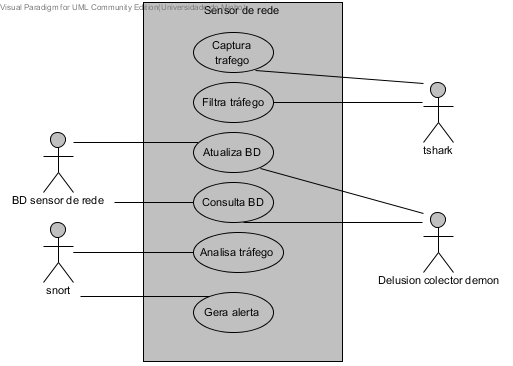
\includegraphics[scale=0.80]{images/ucs/Rede}
	\caption {Diagrama de use case, parte da Rede}
\end{figure}
\pagebreak




\subsubsection{\textbf{3 - Visualizador}}

Descrever aqui o uc da visualizador!!!
\begin{comment}
É possível incluir vários produtos numa mesma simulação. Para o efeito, o utilizador procederá como numa simulação normal, preenchendo os dados correspondentes ao primeiro produto a simular. Terminada esta simulação, é apresentada ao utilizador a opção "acrescentar novo produto (simulação multi-produto)" que, quando seleccionada, agrega a presente simulação à carteira de simulações e apresenta a possibilidade de realização de simulação de um novo produto. 

Repetindo este processo, e quando satisfeito com o número de produtos simulados, o Utilizador solicita o cálculo do prémio conjunto, que tem em conta os descontos aplicáveis a uma simulação multi-produto.
\end{comment}


\begin{figure}[!htb]
	\centering
	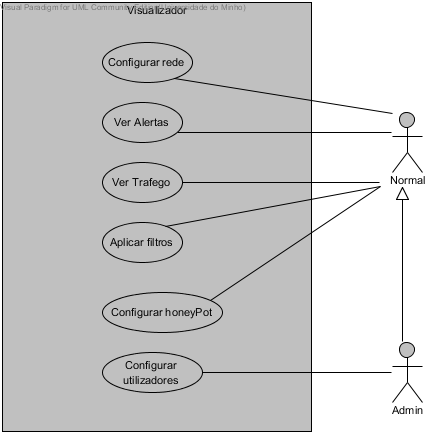
\includegraphics[scale=0.80]{images/ucs/Visualizador}
	\caption {Diagrama de use case, parte da Rede}
\end{figure}
\pagebreak






\subsubsection{\textbf{4 - Configuração HoneyPot}}

Descrever aqui o uc de configuração do honeypot!!!

\begin{comment}
A cada utilizador registado com simulações guardadas será dada a possibilidade de pesquisar pelas mesmas. Tal significa filtrar as simulações guardadas por produto, valor do prémio, etc. O mediador poderá também pesquisar as simulações dos seus clientes. O sistema permite também a consulta das simulações pesquisadas.
\end{comment}

\begin{figure}[!htb]
	\centering
	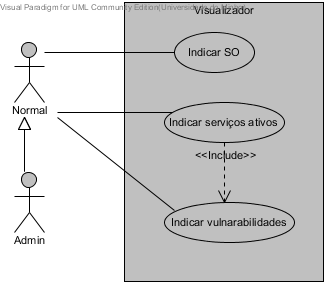
\includegraphics[scale=0.80]{images/ucs/ConfHoneyPot}
	\caption {Diagrama de use case, configuração HoneyPot}
\end{figure}
\pagebreak

\subsubsection{\textbf{5 - Configuração Rede}}

Descrever aqui o uc de configuração de rede!!!

\begin{comment}
A cada utilizador registado com simulações guardadas será dada a possibilidade de pesquisar pelas mesmas. Tal significa filtrar as simulações guardadas por produto, valor do prémio, etc. O mediador poderá também pesquisar as simulações dos seus clientes. O sistema permite também a consulta das simulações pesquisadas.
\end{comment}

\begin{figure}[!htb]
	\centering
	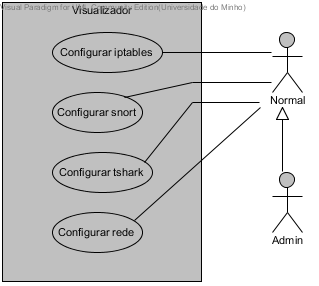
\includegraphics[scale=0.80]{images/ucs/ConfRede}
	\caption {Diagrama de use case, configuração Rede}
\end{figure}
\pagebreak

\subsubsection{\textbf{6 - Configuração Utilizadores}}

Descrever aqui o uc de configuração de utilizadores!!!

\begin{comment}
A cada utilizador registado com simulações guardadas será dada a possibilidade de pesquisar pelas mesmas. Tal significa filtrar as simulações guardadas por produto, valor do prémio, etc. O mediador poderá também pesquisar as simulações dos seus clientes. O sistema permite também a consulta das simulações pesquisadas.
\end{comment}

\begin{figure}[!htb]
	\centering
	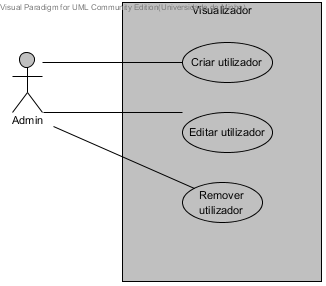
\includegraphics[scale=0.80]{images/ucs/ConfUtilizadores}
	\caption {Diagrama de use case, configuração Utilizadores}
\end{figure}
\pagebreak

